\documentclass{beamer}
\usepackage[utf8]{inputenc}
\usepackage{graphicx, epsfig}
\usepackage{amsmath,mathrsfs,amsfonts,amssymb}
\usepackage{floatflt}
\usepackage{epic,ecltree}
\usepackage{mathtext}
\usepackage{fancybox}
\usepackage{fancyhdr}
\usepackage{multirow}
\usepackage{enumerate}
\usepackage{epstopdf}
\usepackage{multicol}
\usepackage{algorithm}
\usepackage[noend]{algorithmic}
\usepackage{tikz}
\usepackage{blindtext}
\usetheme{default}%{Singapore}%{Warsaw}%{Warsaw}%{Darmstadt}
\usecolortheme{default}

\setbeamerfont{title}{size=\Huge}
\setbeamertemplate{footline}[page number]{}

\setbeamertemplate{section in toc}[sections numbered]


\makeatletter
\newcommand\HUGE{\@setfontsize\Huge{35}{40}}
\makeatother    

\setbeamerfont{title}{size=\HUGE}
\beamertemplatenavigationsymbolsempty

% latin bold lower
\newcommand{\ba}{\mathbf{a}} 
\newcommand{\bc}{\mathbf{c}} 
\newcommand{\be}{\mathbf{e}} 
\newcommand{\bh}{\mathbf{h}} 
\newcommand{\bp}{\mathbf{p}} 
\newcommand{\bt}{\mathbf{t}} 
\newcommand{\bs}{\mathbf{s}} 
\newcommand{\bu}{\mathbf{u}} 
\newcommand{\bv}{\mathbf{v}} 
\newcommand{\bw}{\mathbf{w}} 
\newcommand{\bx}{\mathbf{x}} 
\newcommand{\by}{\mathbf{y}} 
\newcommand{\bz}{\mathbf{z}} 

% latin bold upper
\newcommand{\bA}{\mathbf{A}} 
\newcommand{\bB}{\mathbf{B}} 
\newcommand{\bC}{\mathbf{C}} 
\newcommand{\bI}{\mathbf{I}} 
\newcommand{\bJ}{\mathbf{J}} 
\newcommand{\bL}{\mathbf{L}} 
\newcommand{\bM}{\mathbf{M}} 
\newcommand{\bP}{\mathbf{P}}
\newcommand{\bQ}{\mathbf{Q}} 
\newcommand{\bR}{\mathbf{R}} 
\newcommand{\bT}{\mathbf{T}} 
\newcommand{\bU}{\mathbf{U}} 
\newcommand{\bV}{\mathbf{V}} 
\newcommand{\bW}{\mathbf{W}} 
\newcommand{\bX}{\mathbf{X}} 
\newcommand{\bY}{\mathbf{Y}} 
\newcommand{\bZ}{\mathbf{Z}} 

% latin cal upper
\newcommand{\cF}{\mathcal{F}} 
\newcommand{\cG}{\mathcal{G}} 
\newcommand{\cI}{\mathcal{I}} 
\newcommand{\cL}{\mathcal{L}} 
\newcommand{\cM}{\mathcal{M}} 
\newcommand{\cN}{\mathcal{N}} 
\newcommand{\cP}{\mathcal{P}} 
\newcommand{\cS}{\mathcal{S}} 
\newcommand{\cT}{\mathcal{T}} 
\newcommand{\cW}{\mathcal{W}} 
\newcommand{\cX}{\mathcal{X}} 
\newcommand{\cZ}{\mathcal{Z}} 

% latin bb upper
\newcommand{\bbE}{\mathbb{E}} 
\newcommand{\bbI}{\mathbb{I}} 
\newcommand{\bbP}{\mathbb{P}} 
\newcommand{\bbR}{\mathbb{R}} 

% greek bold lower
\newcommand{\bepsilon}{\boldsymbol{\epsilon}} 
\newcommand{\btheta}{\boldsymbol{\theta}} 
\newcommand{\blambda}{\boldsymbol{\lambda}} 
\newcommand{\bpi}{\boldsymbol{\pi}} 
\newcommand{\bmu}{\boldsymbol{\mu}} 
\newcommand{\bsigma}{\boldsymbol{\sigma}} 
\newcommand{\bphi}{\boldsymbol{\phi}} 

% greek bold upper
\newcommand{\bSigma}{\boldsymbol{\Sigma}} 

\DeclareMathOperator*{\argmin}{arg\,min}
\DeclareMathOperator*{\argmax}{arg\,max}

\newcommand{\createdgmtitle}[1]{\title[\hbox to 56mm{Deep Generative Models  \hfill\insertframenumber\,/\,\inserttotalframenumber}]
	{\vspace{1cm} \\ \textbf{Deep Generative Models} \\ {\Huge Lecture #1}}
	\author{Roman Isachenko}
		\institute{
\includegraphics[width=0.7cm]{../utils/aimasterslogo} \LARGE{AI Masters}}
	\date{2024, Spring}
}

\usepackage{tikz}
\usetikzlibrary{arrows,shapes,positioning,shadows,trees}

\newcommand\myfootnote[1]{%
  \tikz[remember picture,overlay]
  \draw (current page.south west) +(1in + \oddsidemargin,0.5em)
  node[anchor=south west,inner sep=0pt]{\parbox{\textwidth}{%
      \rlap{\rule{10em}{0.4pt}}\raggedright\scriptsize \textit{#1}}};}

\newcommand\myfootnotewithlink[2]{%
  \tikz[remember picture,overlay]
  \draw (current page.south west) +(1in + \oddsidemargin,0.5em)
  node[anchor=south west,inner sep=0pt]{\parbox{\textwidth}{%
      \rlap{\rule{10em}{0.4pt}}\raggedright\scriptsize\href{#1}{\textit{#2}}}};}
      
\AtBeginSection[]
      {
      	\begin{frame}{Outline}
      		\tableofcontents[currentsection]
      	\end{frame}
      }
      \AtBeginSubsection[]{
      	\begin{frame}{Outline}
      		\tableofcontents[currentsection,currentsubsection]
      	\end{frame}
}
\createdgmtitle{13}

\usepackage{tikz}

\usetikzlibrary{arrows,shapes,positioning,shadows,trees}
%--------------------------------------------------------------------------------
\begin{document}
%--------------------------------------------------------------------------------
\begin{frame}[noframenumbering,plain]
%\thispagestyle{empty}
\titlepage
\end{frame}
%=======
\begin{frame}{Recap of previous lecture}
	\begin{block}{Training of DDPM}
		\begin{enumerate}
			\item Get the sample $\bx_0 \sim \pi(\bx)$.
			\item Sample timestamp $t \sim U\{1, T\}$ and the noise $\bepsilon \sim \cN(0, \bI)$.
			\item Get noisy image $\bx_t = \sqrt{\bar{\alpha}_t} \cdot \bx_0 + \sqrt{1 - \bar{\alpha}_t} \cdot \bepsilon$.
			\item Compute loss $ \cL_{\text{simple}} = \| \bepsilon - \bepsilon_{\btheta}(\bx_t , t) \|^2 $.
		\end{enumerate}
	\end{block}
	\begin{block}{Sampling of DDPM}
		\begin{enumerate}
			\item Sample $\bx_T \sim \cN(0, \bI)$.
			\item Compute mean of $p(\bx_{t-1} | \bx_t, \btheta) = \cN(\bmu_{\btheta}(\bx_t, t), \tilde{\beta}_t \bI)$:
			\[
				\bmu_{\btheta}(\bx_t, t) = \frac{1}{\sqrt{\alpha_t}} \cdot \bx_t - \frac{1 - \alpha_t}{\sqrt{\alpha_t (1 - \bar{\alpha}_t)}} \cdot \bepsilon_{\btheta}(\bx_t, t)
			\]
			\vspace{-0.3cm}
			\item Get denoised image $\bx_{t - 1} = \bmu_{\btheta}(\bx_t, t) +  \sqrt{\tilde{\beta}_t} \cdot \bepsilon$, where $\bepsilon \sim \cN(0, \bI)$.
		\end{enumerate}
	\end{block}
	\myfootnotewithlink{https://arxiv.org/abs/2006.11239}{Ho J. Denoising Diffusion Probabilistic Models, 2020}
\end{frame}
%=======
\begin{frame}{Recap of previous lecture}
	\begin{block}{NCSN objective}
		\vspace{-0.2cm}
		\[
			{\color{olive}\bbE_{p(\bx' | \bx, \sigma_t)}}\bigl\| {\color{teal}\bs_{\btheta}(\bx', \sigma_t)} - {\color{violet}\nabla_{\bx'} \log p(\bx' | \bx, \sigma_t)} \bigr\|^2_2 \rightarrow \min_{\btheta}
		\]
	\end{block}
	\vspace{-0.3cm}
	\begin{block}{DDPM objective}
		\vspace{-0.2cm}
		\[
			\cL_t = {\color{olive}\bbE_{\bepsilon \sim \cN(0, \bI)}} \left[ \frac{(1 - \alpha_t)^2}{2\tilde{\beta}_t \alpha_t} \left\| {\color{violet}\frac{\bepsilon}{\sqrt{1 - \bar{\alpha}_t}}} - {\color{teal}\frac{\bepsilon_{\btheta}(\bx_t, t)}{\sqrt{1 - \bar{\alpha}_t}}}\right\|^2 \right]
		\]
		\vspace{-0.7cm}
	\end{block}
	\begin{align*}
		q(\bx_t | \bx_0) &= \cN(\sqrt{\bar{\alpha}_t} \cdot \bx_0, (1 - \bar{\alpha}_t) \cdot \bI) \\
		{\color{violet}\nabla_{\bx_t} \log q(\bx_t | \bx_0)} &= - \frac{\bx_t - \sqrt{\bar{\alpha}_t} \cdot \bx_0}{1 - \bar{\alpha}_t} = - \frac{\bepsilon}{\sqrt{1 - \bar{\alpha}_t}}.
	\end{align*}
		Let reparametrize our model: 
		\vspace{-0.2cm}
		\[
			{\color{teal}\bs_{\btheta}(\bx_t, t)} = - \frac{\bepsilon_{\btheta}(\bx_t, t)}{\sqrt{1 - \bar{\alpha}_t}}.
		\]
	\myfootnotewithlink{https://arxiv.org/abs/2006.11239}{Ho J. Denoising Diffusion Probabilistic Models, 2020}
	\end{frame}
%=======
\begin{frame}{Outline}
	\tableofcontents
\end{frame}
%=======
\section{SDE basics}
%=======
\begin{frame}{Stochastic differential equation (SDE)}
	Let define stochastic process $\bx(t)$ with initial condition $\bx(0) \sim p_0(\bx)$:
	\[
		d\bx = \mathbf{f}(\bx, t) dt + g(t) d \bw
	\]
	\vspace{-0.6cm}
	\begin{itemize}
		 \item $\mathbf{f}(\bx, t)$ is the \textbf{drift} function of $\bx(t)$.
		 \item $g(t)$ is the \textbf{diffusion} coefficient of $\bx(t)$.
		 \item If $g(t) = 0$ we get standard ODE.
		 \item $\bw(t)$ is the standard Wiener process (Brownian motion):
		 \begin{enumerate}
		 	\item $\bw(0) = 0$ (almost surely);
		 	\item $\bw(t)$ has independent increments;
			 \item $\bw(t) - \bw(s) \sim \cN(0, (t - s) \bI)$.
		 \end{enumerate}
		 \item $d \bw = \bw(t + dt) - \bw(t) = \cN(0, \bI \cdot dt ) = \bepsilon \cdot \sqrt{dt}$, where $\bepsilon \sim \cN(0, \bI)$.
	\end{itemize}
	\textbf{Note:} In contrast to ODE, initial condition $\bx(0)$ does not uniquely determine the process trajectory.
\end{frame}
%=======
\begin{frame}{Stochastic differential equation (SDE)}
	\vspace{-0.4cm}
	\[
		d\bx = \mathbf{f}(\bx, t) dt + g(t) d \bw, \quad d \bw = \bepsilon \cdot \sqrt{dt}, \quad \bepsilon \sim \cN(0, \bI).
	\]
	\vspace{-0.4cm}
	\begin{itemize}
		\item At each moment $t$ we have the density $p(\bx(t), t)$.
		\item How to get distribution $p(\bx, t)$ for $\bx(t)$?
	\end{itemize}
 	\begin{block}{Theorem (Kolmogorov-Fokker-Planck)}
 		Evolution of the distribution $p(\bx, t)$ is given by the following ODE:
 		\vspace{-0.2cm}
 		\[
 			\frac{\partial p(\bx, t)}{\partial t} = \text{tr}\left(- \frac{\partial}{\partial \bx} \bigl[ \mathbf{f}(\bx, t) p(\bx, t)\bigr] + \frac{1}{2} g^2(t) \frac{\partial^2 p(\bx, t)}{\partial \bx^2} \right)
 		\]
 		\textbf{Note:} This is the generalization of KFP theorem that we used in continuous-in-time NF.
 	\end{block}
 	\begin{block}{Langevin SDE (special case)}
 		\vspace{-0.6cm}
 		\begin{align*}
 			d\bx &= {\color{violet}\mathbf{f}(\bx, t)} dt + {\color{teal}g(t)} d \bw \\
 			d \bx &= {\color{violet}\frac{1}{2} \frac{\partial}{\partial \bx} \log p(\bx, t)} d t + {\color{teal} 1 } \cdot d \bw
 		\end{align*}
 	\end{block}
\end{frame}
%=======
\begin{frame}{Langevin SDE (special case)}
	\[
		d \bx = {\color{violet}\frac{1}{2} \frac{\partial}{\partial \bx} \log p(\bx, t)} d t + {\color{teal} 1 } \cdot d \bw
	\]
	Let apply KFP theorem.
	\begin{multline*}
		\frac{\partial p(\bx, t)}{\partial t} =  \text{tr} \left(- \frac{\partial}{\partial \bx}\left[ {\color{olive}p(\bx, t) \frac{1}{2} \frac{\partial}{\partial \bx} \log p(\bx, t)} \right]  + \frac{1}{2} \frac{\partial^2 p(\bx, t)}{\partial \bx^2} \right) = \\
		= \text{tr} \left(- \frac{\partial}{\partial \bx}\left[ {\color{olive}\frac{1}{2} \frac{\partial}{\partial \bx} p(\bx, t) } \right]  + \frac{1}{2} \frac{\partial^2 p(\bx, t)}{\partial \bx^2} \right) = 0
	\end{multline*}
	The density $p(\bx, t) = \text{const}(t)$! \\
	\begin{block}{Discretized Langevin SDE}
		\vspace{-0.3cm}
		\[
			\bx_{t + 1} - \bx_t = \frac{\eta}{2} \cdot \frac{\partial}{\partial \bx} \log p(\bx, t) + \sqrt{\eta} \cdot \bepsilon, \quad \eta \approx dt.
		\]
		\vspace{-0.4cm}
	\end{block}
	\begin{block}{Langevin dynamic}
		\vspace{-0.3cm}
		\[
			\bx_{t + 1} = \bx_t + \frac{\eta}{2} \cdot \nabla_{\bx} \log p(\bx | \btheta) + \sqrt{\eta} \cdot \bepsilon, \quad \eta \approx dt.
		\]
		\vspace{-0.3cm}
	\end{block}
\end{frame}
%=======
\section{Diffusion and Score matching SDEs}
%=======
\begin{frame}{Score matching SDE}
	\begin{block}{Denoising score matching}
		\vspace{-0.7cm}
		\begin{align*}
			\bx_l &= \bx + \sigma_l \cdot \bepsilon_l, \quad p(\bx_l | \bx, \sigma_l) = \cN(\bx, \sigma_l^2 \bI) \\
			\bx_{l-1} &= \bx + \sigma_{l-1} \cdot \bepsilon_{l-1}, \quad p(\bx_{l-1} | \bx, \sigma_{l-1}) = \cN(\bx, \sigma_{l-1}^2 \bI)
		\end{align*}
	\end{block}
	\vspace{-0.7cm}
	\[
		\bx_l = \bx_{l - 1} + \sqrt{\sigma^2_l - \sigma^2_{l-1}} \cdot \bepsilon, \quad p(\bx_l | \bx_{l-1}, \sigma_l) = \cN(\bx_{l-1}, (\sigma_l^2 - \sigma_{l-1}^2) \cdot \bI)
	\]
	Let turn this Markov chain to the continuous stochastic process~$\bx(t)$ taking $L \rightarrow \infty$:
	\[
		{\color{teal}\bx(t + dt)} = {\color{teal}\bx(t)} + \sqrt{\frac{\sigma^2(t + dt) - \sigma^2(t)}{dt} {\color{violet}dt}} \cdot {\color{violet}\bepsilon} = \bx(t) + \sqrt{\frac{ d [\sigma^2(t)]}{dt}} \cdot {\color{violet}d \bw}
	\]
	\vspace{-0.5cm}
	\begin{block}{Variance Exploding SDE}
		\vspace{-0.3cm}
		\[
			d \bx = \sqrt{\frac{ d [\sigma^2(t)]}{dt}} \cdot d \bw
		\]
	\end{block}
	\myfootnotewithlink{https://arxiv.org/abs/2011.13456}{Song Y., et al. Score-Based Generative Modeling through Stochastic Differential Equations, 2020}
\end{frame}
%=======
\begin{frame}{Diffusion SDE}
	\begin{block}{Denoising Diffusion}
		\vspace{-0.5cm}
		\[
			\bx_t = \sqrt{1 - \beta_t} \cdot \bx_{t - 1} + \sqrt{\beta_t} \cdot \bepsilon, \quad q(\bx_t | \bx_{t-1}) = \cN(\sqrt{1 - \beta_t} \cdot \bx_{t-1}, \beta_t \cdot \bI)
		\]
		\vspace{-0.5cm}
	\end{block}
	Let turn this Markov chain to the continuous stochastic process taking $T \rightarrow \infty$ and taking $\beta(\frac{t}{T}) = \beta_t \cdot T$
	\begin{multline*}
		{\color{teal}\bx(t)} = \sqrt{1 - \beta(t) dt} \cdot \bx(t - dt) + \sqrt{\beta(t)dt} \cdot \bepsilon \approx \\
		\approx (1 - \frac{1}{2} \beta(t) dt) \cdot \bx(t - dt) + \sqrt{\beta(t){\color{violet}dt}} \cdot {\color{violet}\bepsilon} = \\
		= {\color{teal}\bx(t - dt)} - \frac{1}{2} \beta(t) \bx(t - dt) dt  + \sqrt{\beta(t)} \cdot {\color{violet}d \bw}
	\end{multline*}
	\vspace{-0.5cm}
	\begin{block}{Variance Preserving SDE}
		\vspace{-0.3cm}
		\[
			{\color{teal}d \bx} = - \frac{1}{2} \beta(t) \bx(t) dt + \sqrt{\beta(t)} \cdot d \bw
		\]
	\end{block}
	\myfootnotewithlink{https://arxiv.org/abs/2011.13456}{Song Y., et al. Score-Based Generative Modeling through Stochastic Differential Equations, 2020}
\end{frame}
%=======
\begin{frame}{Diffusion SDE}
	\begin{figure}
		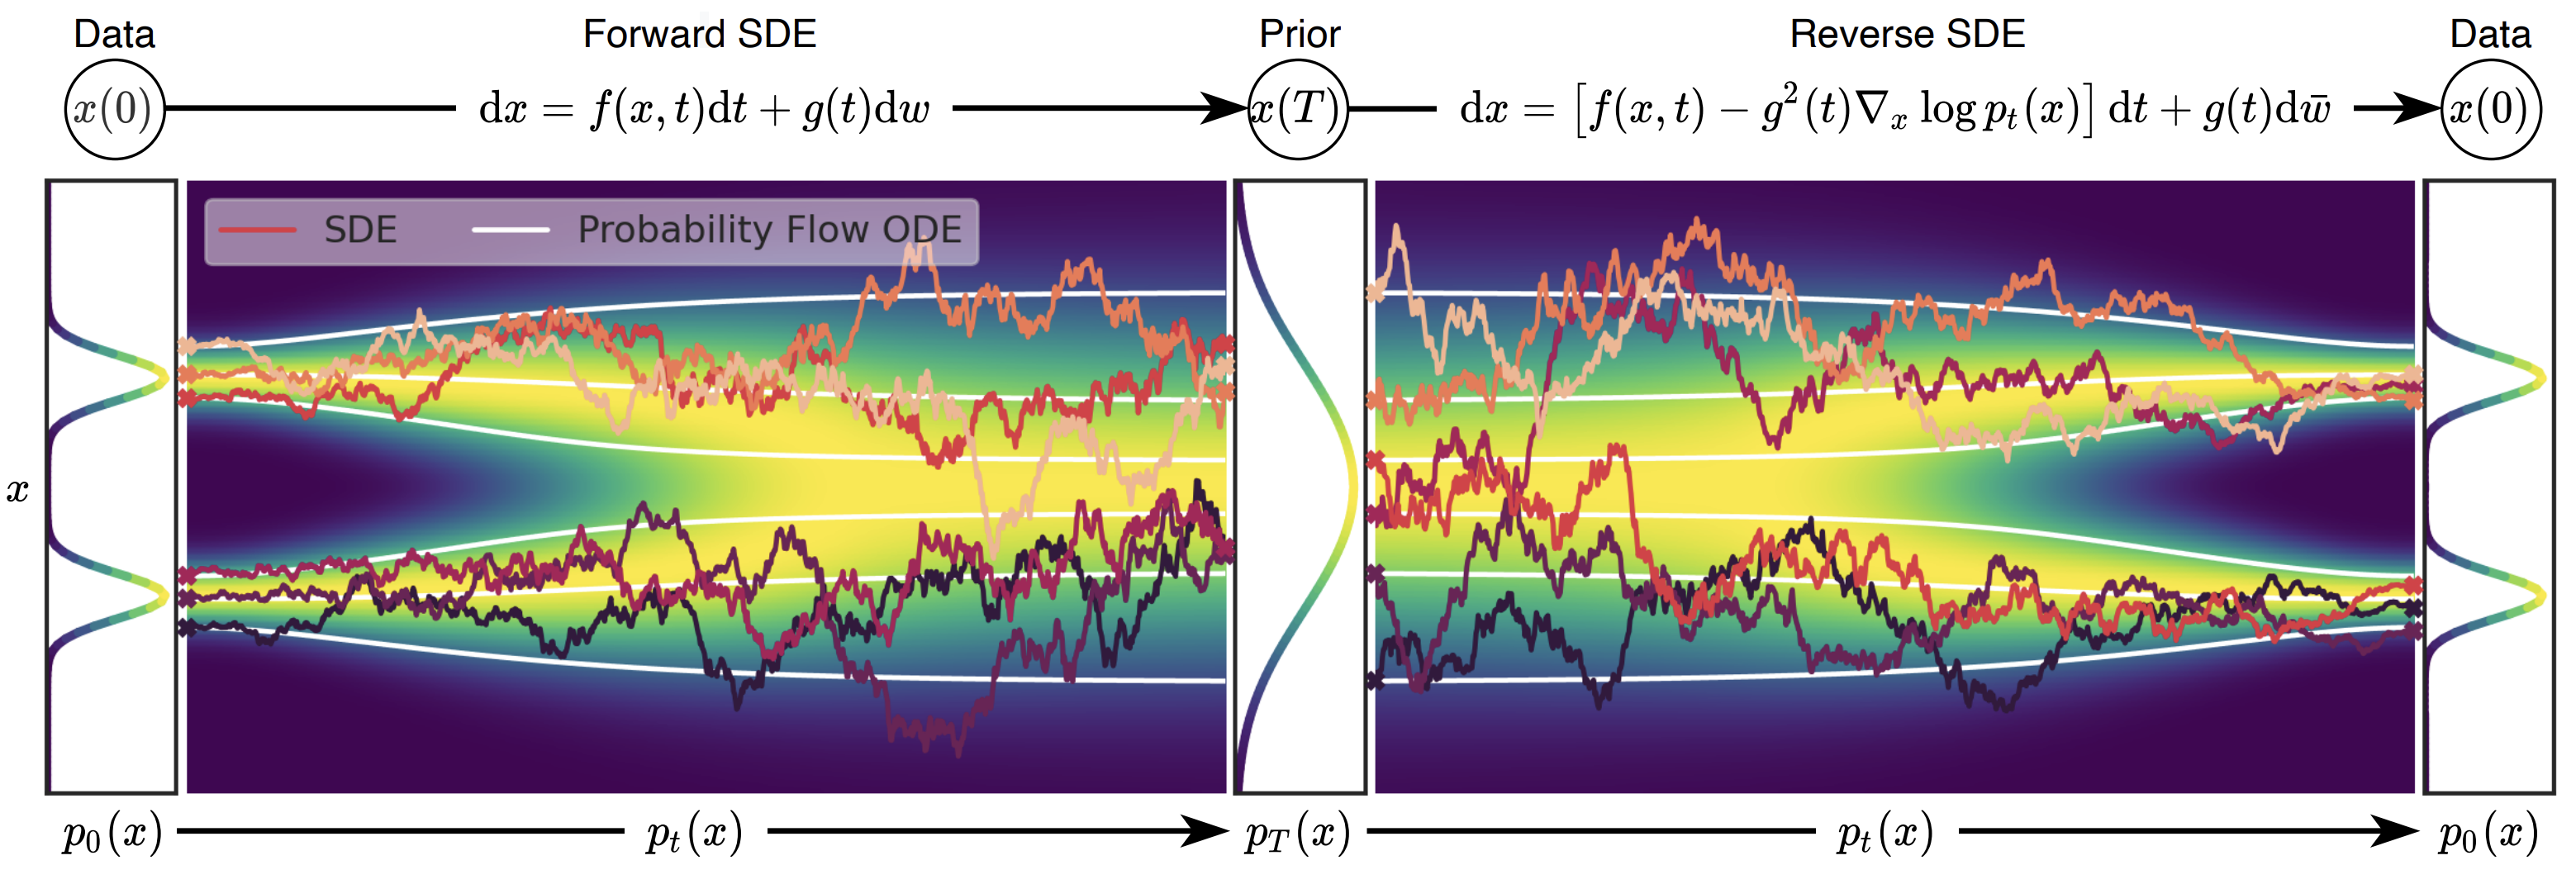
\includegraphics[width=\linewidth]{figs/sde}
	\end{figure}
	\vspace{-0.3cm}
	\begin{block}{Variance Exploding SDE (NCSN)}
		\vspace{-0.3cm}
		\[
			d \bx = \sqrt{\frac{ d [\sigma^2(t)]}{dt}} \cdot d \bw
		\]
		\vspace{-0.3cm}
	\end{block}
	\begin{block}{Variance Preserving SDE (DDPM)}
		\vspace{-0.3cm}
		\[
			d \bx = - \frac{1}{2} \beta(t) \bx(t) dt + \sqrt{\beta(t)} \cdot d \bw
		\]
	\end{block}
	\myfootnotewithlink{https://arxiv.org/abs/2011.13456}{Song Y., et al. Score-Based Generative Modeling through Stochastic Differential Equations, 2020}
\end{frame}
%=======
\begin{frame}{Summary}
	\begin{itemize}
		\item Score matching (NCSN) and diffusion models (DDPM) are the discretizations of the SDEs (variance exploding and variance preserving).
	\end{itemize}
\end{frame}
\end{document} 